% Active cross-modal architecture -- pictorial version.
% Every block uses a FIXED text width, so node boxes cannot grow into one
% another; all x-ranges below are disjoint by construction.
%   image  -1.15..1.15 | encoders 2.15..5.05 | cross 5.95..8.85
%   heads   9.35..10.65 | fusion  11.15..14.05 | output 14.50..17.50
% Requires graphicx, fontawesome5, TikZ libraries arrows.meta, positioning, fit.
\begin{tikzpicture}[
  font=\small,
  >={Stealth[length=2.6mm,width=1.9mm]},
  flow/.style={->, thick, draw=black!70},
  aux/.style={->, semithick, dashed, draw=headblue},
  blk/.style={draw=black!48, rounded corners=4pt, thick, fill=white,
              align=center, inner sep=5pt},
  chip/.style={draw=black!32, rounded corners=3pt, fill=white,
               inner xsep=4pt, inner ysep=2pt, font=\scriptsize, align=center}
]

%============================================================ offline controls
\draw[headblue, dashed, rounded corners=4pt, fill=blue!3, line width=0.7pt]
  (-1.15,2.95) rectangle (17.50,3.75);
\node[anchor=west, font=\scriptsize] at (-0.95,3.35)
  {{\color{headblue}\faLock}~\textbf{Offline controls}};
\node[chip, anchor=west, fill=blue!5] at (2.05,3.35)
  {\faLayerGroup~source-group split};
\node[chip, anchor=west, fill=blue!5] at (5.55,3.35) {\faKey~exact box key};
\node[chip, anchor=west, fill=blue!5] at (8.35,3.35) {\faFilter~178-token mask};
\node[chip, anchor=west, fill=green!6, draw=green!45!black] at (11.55,3.35)
  {\checkmark~validation-only selection: \textbf{89.19\%} $>$ 82.43\%};

%============================================================ inputs
\node[blk, text width=1.95cm, minimum height=1.70cm, fill=vitgreen!25]
  (image) at (0,1.35) {};
\node[inner sep=0.4pt, draw=black!30] at (0,1.28)
  {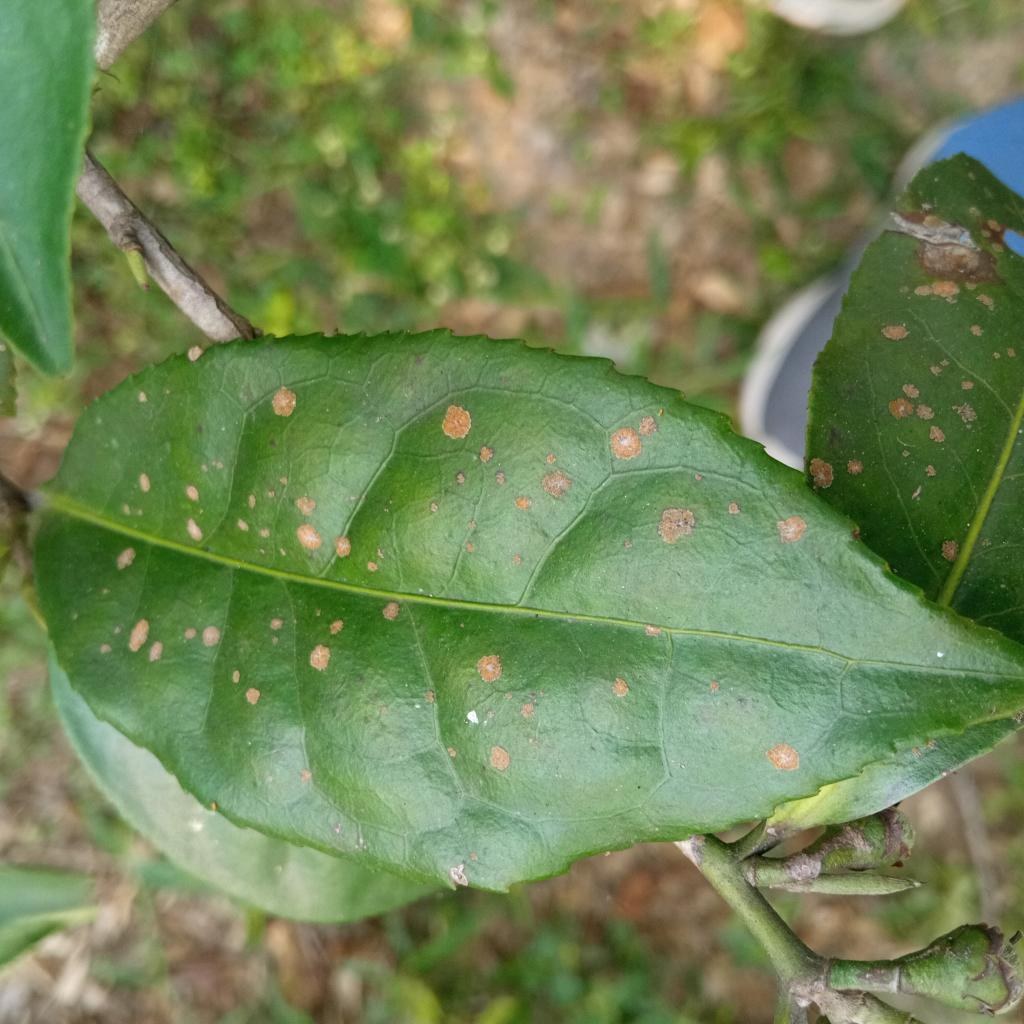
\includegraphics[width=1.62cm,height=1.00cm,keepaspectratio]
   {data_final/data_final/real_dataset_sorted/LEAF_RUST/107_jpg.rf.9c0264c78b1f4dfff87adea98349df8b.jpg}};
\node[font=\small\bfseries, anchor=south] at (0,2.24)
  {{\color{green!45!black}\faImage}~Leaf crop};
\node[chip, anchor=north] at (0,0.46) {$224\times224$};

\node[blk, text width=1.95cm, minimum height=1.70cm, fill=outyyellow]
  (text) at (0,-1.35) {};
\node[draw=black!40, fill=white, minimum width=1.62cm, align=left,
      font=\scriptsize, inner sep=3pt] at (0,-1.30)
  {scattered spots\\powdery texture\\tip affected};
\node[font=\small\bfseries, anchor=south] at (0,-0.46)
  {{\color{orange!70!black}\faStickyNote}~Field note};
\node[chip, anchor=north] at (0,-2.26) {$\leq 128$ tokens};

%============================================================ encoders
\node[blk, text width=2.60cm, minimum height=1.70cm, fill=smallgray!60]
  (vision) at (3.60,1.35)
  {{\Large\color{headblue}\faSnowflake}\,{\Large\color{black!55}\faLayerGroup}\\[2pt]
   {\small\bfseries Frozen ResNet-50}\\
   {\scriptsize\color{black!70} $49\times256$ tokens}};

\node[blk, text width=2.60cm, minimum height=1.70cm, fill=llmblue!45]
  (language) at (3.60,-1.35)
  {{\Large\color{headblue}\faFont}\,{\Large\color{black!55}\faProjectDiagram}\\[2pt]
   {\small\bfseries Text Transformer}\\
   {\scriptsize\color{black!70} 2 layers $\cdot$ 4 heads}};

%============================================================ cross-attention
\node[blk, text width=2.60cm, minimum height=3.30cm, fill=vlmred!20]
  (cross) at (7.40,0)
  {{\small\bfseries Cross-attention}\\
   {\scriptsize\color{black!70} 8 heads, both ways}\\[7pt]
   \begin{tikzpicture}[baseline=-0.6ex]
     \foreach \y in {-0.52,-0.26,0,0.26,0.52}{
       \fill[headblue]        (-0.68,\y) circle (0.085);
       \fill[orange!85!black] ( 0.68,\y) circle (0.085);
     }
     \foreach \a/\b in {-0.52/0, -0.26/0.52, 0.26/-0.26}{
       \draw[headblue, line width=0.7pt, opacity=0.9] (-0.60,\a)--(0.60,\b);
     }
     \foreach \a/\b in {0.52/-0.26, 0/0.26, -0.26/-0.52}{
       \draw[orange!85!black, line width=0.7pt, opacity=0.9] (0.60,\a)--(-0.60,\b);
     }
     \node[font=\scriptsize, text=headblue]        at (-0.68,0.86) {$H_t$};
     \node[font=\scriptsize, text=orange!75!black] at ( 0.68,0.86) {$H_v$};
   \end{tikzpicture}};

%============================================================ expert heads
\node[blk, text width=0.95cm, minimum height=0.62cm, fill=smallgray!50,
      font=\scriptsize, inner sep=3pt] (vhead) at (10.00,0.85)
  {{\color{green!40!black}\faImage}~$z_v$};
\node[blk, text width=0.95cm, minimum height=0.62cm, fill=llmblue!35,
      font=\scriptsize, inner sep=3pt] (thead) at (10.00,-0.85)
  {{\color{headblue}\faFont}~$z_t$};

%============================================================ fusion
\node[blk, text width=2.60cm, minimum height=3.30cm, fill=fedorange!60]
  (fusion) at (12.60,0)
  {{\small\bfseries Reliability fusion}\\[7pt]
   \begin{tikzpicture}[baseline=-0.6ex]
     \fill[headblue!75, rounded corners=1pt] (-1.10,-0.15) rectangle (0.17,0.15);
     \fill[orange!80!black, rounded corners=1pt] (0.17,-0.15) rectangle (1.10,0.15);
     \draw[black!55, rounded corners=1pt, line width=0.5pt]
       (-1.10,-0.15) rectangle (1.10,0.15);
     \node[font=\tiny, text=white] at (-0.47,0) {$r_t\,0.575$};
     \node[font=\tiny, text=white] at ( 0.63,0) {$r_v\,0.425$};
   \end{tikzpicture}\\[7pt]
   {\scriptsize\color{black!70} $r_t+r_v=1$}\\[2pt]
   {\scriptsize\color{black!70} $+$ residual $\lambda=2$}};

%============================================================ output
\node[blk, text width=2.70cm, minimum height=3.30cm, fill=vitgreen!30]
  (output) at (16.00,0) {};
\node[font=\small\bfseries] at (16.00,1.28)
  {{\color{green!45!black}\faChartLine}~Five-class head};
\foreach \i/\lab/\ww/\cc in {0/Blight/1.30/headblue, 1/Hoppers/0.42/black!45,
                             2/Rust/0.92/green!55!black, 3/Looper/0.64/orange!85!black,
                             4/{Mosq.}/0.34/vlmred}{
  \node[font=\tiny, anchor=east] at (15.42,0.70-0.36*\i) {\lab};
  \draw[fill=black!10, draw=none] (15.50,0.60-0.36*\i) rectangle (17.10,0.80-0.36*\i);
  \draw[fill=\cc, draw=none] (15.50,0.60-0.36*\i) rectangle (15.50+\ww,0.80-0.36*\i);
}
\node[chip, anchor=north] at (16.00,-1.02) {$p(y\mid x,t)$};

%============================================================ runtime flow
\draw[flow] (image.east)    -- (vision.west);
\draw[flow] (text.east)     -- (language.west);
\draw[flow] (vision.east)   -- (5.95,1.35);
\draw[flow] (language.east) -- (5.95,-1.35);
\draw[flow] (cross.east)    -- (fusion.west);
\draw[flow] (fusion.east)   -- (output.west);

% expert heads: branch above/below the cross block, never through it
\draw[aux] (vision.east)   -- (5.40,1.35) -- (5.40,2.08) -- (10.00,2.08)
           -- (vhead.north);
\draw[aux] (language.east) -- (5.40,-1.35) -- (5.40,-2.08) -- (10.00,-2.08)
           -- (thead.south);
\draw[aux] (vhead.east) -- ([yshift=0.85cm]fusion.west);
\draw[aux] (thead.east) -- ([yshift=-0.85cm]fusion.west);

% offline controls govern the input stage and the fused core
\draw[dashed, draw=headblue, -{Stealth[length=1.8mm]}] (0,2.95) -- (0,2.52);
\draw[dashed, draw=headblue, -{Stealth[length=1.8mm]}] (12.60,2.95) -- (12.60,1.70);

\end{tikzpicture}
